% ----------------------------------------------------------
% Capítulo de Resultados
% ----------------------------------------------------------
\chapter{Resultados e Validação}
\label{cap:resultados}
% ---

Este capítulo apresenta os resultados obtidos com o desenvolvimento do sistema, focando na validação das regras de negócio através de testes automatizados e na análise de desempenho da interface do usuário.

A qualidade do software foi verificada em duas frentes: a integridade do \textit{backend}, garantida por testes de unidade e integração utilizando o \textit{framework} PHPUnit, e a eficiência do \textit{frontend}, medida através da ferramenta Google Lighthouse.

\section{Testes Automatizados de Backend}
\label{sec:testes-backend}

Para garantir a robustez das operações críticas do sistema, como o controle de estoque e o isolamento de dados entre diferentes usuários (multitenancy), foram implementadas suítes de testes automatizados. Abaixo são detalhados os principais cenários validados.

\subsection{Integridade do Estoque}

Um dos requisitos mais críticos do sistema é impedir que produtos sejam movimentados sem saldo suficiente. O teste de integridade de estoque (`EstoqueIntegridadeTest`) valida que o sistema lança uma exceção ao tentar realizar uma saída maior que a quantidade disponível.

O código a seguir demonstra a validação dessa regra de negócio diretamente na camada de serviço:

\begin{verbatim}
// Teste: Não deve permitir saída de estoque insuficiente
public function test_nao_deve_permitir_saida_de_estoque_insuficiente()
{
    $user = User::factory()->create();
    $produto = Produto::factory()->create([
        'user_id' => $user->id,
        'quantidade_estoque' => 5
    ]);

    $service = new EstoqueService();

    // Espera-se que o sistema bloqueie a operação
    $this->expectException(Exception::class);
    $this->expectExceptionMessage('Estoque insuficiente para esta saída.');

    $service->movimentarEstoque($produto, 'saida', 10);
}
\end{verbatim}

\subsection{Fluxo de Vendas}

O teste de fluxo de vendas (`VendaFluxoTest`) simula uma transação completa via API. Ele verifica se, ao finalizar uma venda, o sistema realiza três ações simultâneas corretamente: o registro da venda, o cálculo do valor total e a baixa automática no estoque dos produtos envolvidos.

O cenário de teste implementado garante que:
\begin{enumerate}
    \item O sistema aceita a venda via requisição HTTP;
    \item O total da venda é calculado corretamente (soma dos produtos);
    \item A quantidade em estoque dos produtos vendidos é decrementada no banco de dados.
\end{enumerate}

\subsection{Segurança e Isolamento de Dados}

Considerando que a aplicação pode ser utilizada por múltiplos microempreendedores (MEIs), a segurança dos dados é fundamental. O teste `SegurancaDadosTest` valida o isolamento das informações, garantindo que um usuário autenticado não consiga visualizar, editar ou excluir dados pertencentes a outro usuário.

\begin{verbatim}
public function test_usuario_nao_pode_ver_produtos_de_outro_usuario()
{
    // Usuário A (Dono do produto) cria um produto
    $userA = User::factory()->create();
    $produtoA = Produto::factory()->create([
        'user_id' => $userA->id, 
        'nome' => 'Produto Secreto'
    ]);

    // Usuário B (Intruso) tenta acessar
    $userB = User::factory()->create();
    $this->actingAs($userB);

    // Tenta listar produtos
    $response = $this->getJson('/api/produtos');

    // O JSON retornado NÃO deve conter o produto do Usuário A
    $response->assertJsonMissing(['nome' => 'Produto Secreto']);
}
\end{verbatim}

Essa validação garante a privacidade das informações financeiras e de estoque de cada MEI cadastrado na plataforma.

\subsection{Conclusão dos Testes de Backend}

A execução bem-sucedida da suíte de testes automatizados valida a robustez e a confiabilidade das regras de negócio implementadas no \textit{backend}. A cobertura de cenários críticos — abrangendo desde a integridade das transações de estoque até o isolamento rigoroso dos dados entre diferentes usuários — assegura que o sistema opera de maneira consistente e segura.

Como evidenciado na Figura \ref{fig:testes-geral}, todos os testes foram concluídos com êxito, confirmando que a lógica da aplicação atende plenamente aos requisitos funcionais e de segurança estabelecidos. Essa validação estrutural do servidor fornece a base necessária para garantir uma experiência de usuário estável, permitindo que a avaliação do sistema avance para os aspectos de desempenho e interface, conforme abordado na seção a seguir.

\begin{figure}[htb]
    \caption{\label{fig:testes-geral}Relatório de execução dos testes automatizados}
    \begin{center}
        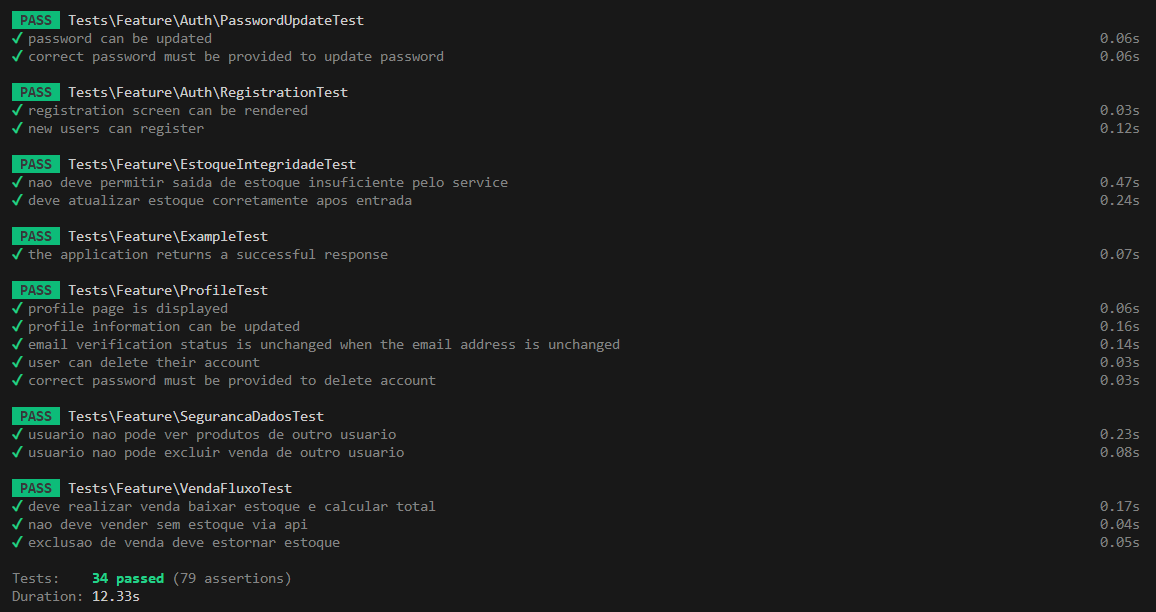
\includegraphics[width=1.0\textwidth]{img/testes-backend-geral}
    \end{center}
    \legend{Fonte: Elaborado pelo autor.}
\end{figure}

\section{Análise de Desempenho e Qualidade (Frontend)}
\label{sec:lighthouse}

A interface do sistema foi submetida à auditoria do Google Lighthouse, uma ferramenta automatizada de código aberto para melhorar a qualidade de páginas web. A auditoria avalia métricas de desempenho, acessibilidade, boas práticas e SEO (\textit{Search Engine Optimization}).

Os resultados obtidos demonstram a eficácia da escolha da \textit{stack} tecnológica (React e Inertia.js) e das otimizações implementadas. Como pode ser observado na Figura \ref{fig:lighthouse}, o sistema obteve pontuação máxima (100) em "Best Practices" e "SEO", além de resultados excelentes em Performance (98) e Acessibilidade (97).

\begin{figure}[htb]
    \caption{\label{fig:lighthouse}Resultado da auditoria Google Lighthouse}
    \begin{center}
        % IMPORTANTE: Salve o seu print como 'lighthouse-result.png' na pasta 'img'
        % Se a imagem não aparecer, verifique se o nome do arquivo está exato.
        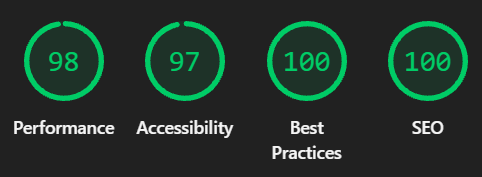
\includegraphics[width=1.0\textwidth]{img/lighthouse-result}
    \end{center}
    \legend{Fonte: Elaborado pelo autor com base na ferramenta Google Lighthouse (2025).}
\end{figure}

O alto desempenho é atribuído ao uso de carregamento assíncrono para componentes pesados e à renderização eficiente do \textit{Virtual DOM} do React. A acessibilidade foi garantida através do uso de tags semânticas HTML5 e atributos ARIA adequados nos componentes de interface.

\subsection{Interfaces do Sistema}

Abaixo são apresentadas as telas principais do sistema desenvolvido, evidenciando a usabilidade e a aplicação da identidade visual proposta.

\begin{figure}[htb]
    \caption{\label{fig:dashboard}Painel de Controle (Dashboard) do Sistema}
    \begin{center}
        % Substitua 'dashboard' pelo nome do arquivo do seu print do dashboard
        
\includegraphics[width=1.0\textwidth]{dashboard}
    \end{center}
    \legend{Fonte: Elaborado pelo autor.}
\end{figure}

\begin{figure}[htb]
    \caption{\label{fig:vendas}Tela de Realização de Vendas}
    \begin{center}
        % Substitua 'vendas' pelo nome do arquivo do seu print de vendas
        \includegraphics[width=1.0\textwidth]{vendas}
    \end{center}
    \legend{Fonte: Elaborado pelo autor.}
\end{figure}